\documentclass{article}

\usepackage{amsmath}
\usepackage{amssymb}
\usepackage{bm}
\usepackage{color}
\usepackage{CJKutf8}
\usepackage{color}
\usepackage{enumitem}
\usepackage{graphicx}
\usepackage{indentfirst}
\usepackage{listings}
\usepackage{mathdots}
\usepackage{tikz}
\usepackage{wasysym}
\usepackage{xcolor}

\setlength{\parindent}{2em}

\usetikzlibrary{shapes,arrows, automata}

\allowdisplaybreaks

\newcommand{\hytt}[1]{\texttt{\hyphenchar\font=\defaulthyphenchar #1}}
\hyphenation{read-Sym-bol re-ad-Space-Tab-New-line str-Tab}

\definecolor{mygreen}{rgb}{0,0.6,0}
\definecolor{mygray}{rgb}{0.5,0.5,0.5}
\definecolor{mymauve}{rgb}{0.58,0,0.82}
%\footnotesize
\lstset{ %
  backgroundcolor=\color{white},   % choose the background color; you must add \usepackage{color} or \usepackage{xcolor}
  basicstyle=\ttfamily,            % the size of the fonts that are used for the code
  breakatwhitespace=false,         % sets if automatic breaks should only happen at whitespace
  breaklines=true,                 % sets automatic line breaking
  captionpos=b,                    % sets the caption-position to bottom
  commentstyle=\ttfamily\color{mygreen},    
                                   % comment style
  deletekeywords={},               % if you want to delete keywords from the given language
  escapeinside={},                 % if you want to add LaTeX within your code
  extendedchars=true,              % lets you use non-ASCII characters; for 8-bits encodings only, does not work with UTF-8
  frame=single,                    % adds a frame around the code
  keepspaces=true,                 % keeps spaces in text, useful for keeping indentation of code (possibly needs columns=flexible)
  keywordstyle=\color{blue},       % keyword style
  language=VHDL,                    % the language of the code
  morekeywords={},                 % if you want to add more keywords to the set
  numbers=left,                    % where to put the line-numbers; possible values are (none, left, right)
  numbersep=5pt,                   % how far the line-numbers are from the code
  numberstyle=\tiny\color{mygray}, % the style that is used for the line-numbers
  rulecolor=\color{black},         % if not set, the frame-color may be changed on line-breaks within not-black text (e.g. comments (green here))
  showspaces=false,                % show spaces everywhere adding particular underscores; it overrides 'showstringspaces'
  showstringspaces=false,          % underline spaces within strings only
  showtabs=false,                  % show tabs within strings adding particular underscores
  stepnumber=1,                    % the step between two line-numbers. If it's 1, each line will be numbered
  stringstyle=\color{mymauve},     % string literal style
  tabsize=2,                       % sets default tabsize to 2 spaces
  title=\lstname                   % show the filename of files included with \lstinputlisting; also try caption instead of title
}

\begin{document}
\begin{CJK*}{UTF8}{gbsn}
\CJKtilde

\title{实验二(2) 加法器设计实验}

\author{计算机1202 张艺瀚\\学号:20123852}
\maketitle

\section{实验目的}
\begin{enumerate}
\item 学习了解加法器工作原理。
\item 学习用VHDL语言设计全加器的设计方法。
\item 学习使用元件例化的方法设计多位加法器。
\end{enumerate}

\section{实验原理}
两个n位二进制数相加的过程,是从最低有效位开始相加,形成和数并传送进位最后得到结果。最低位只有加数和被加数相加,这种两个一位数相加称为半加;完成加数,被加数,低位的进位数三个一位数相加称为全加。实现半加运算的电路称为半加器,实现全加运算的电路称为全加器。

全加器(Full Adder)的真值表如下表所示,其中$C_i$是低位进位,$C_{i+1}$是向高位的进位。

全加器真值表如图~\ref{fig: true} 所示。
\begin{center}
\begin{figure}[h!]
\includegraphics[width=\textwidth]{true.jpg}
\caption{全加器真值表}
\label{fig: true}
\end{figure}
\end{center}

全加器(Full Adder)的逻辑图请参考图~\ref{fig: logic}。
\begin{center}
\begin{figure}[h!]
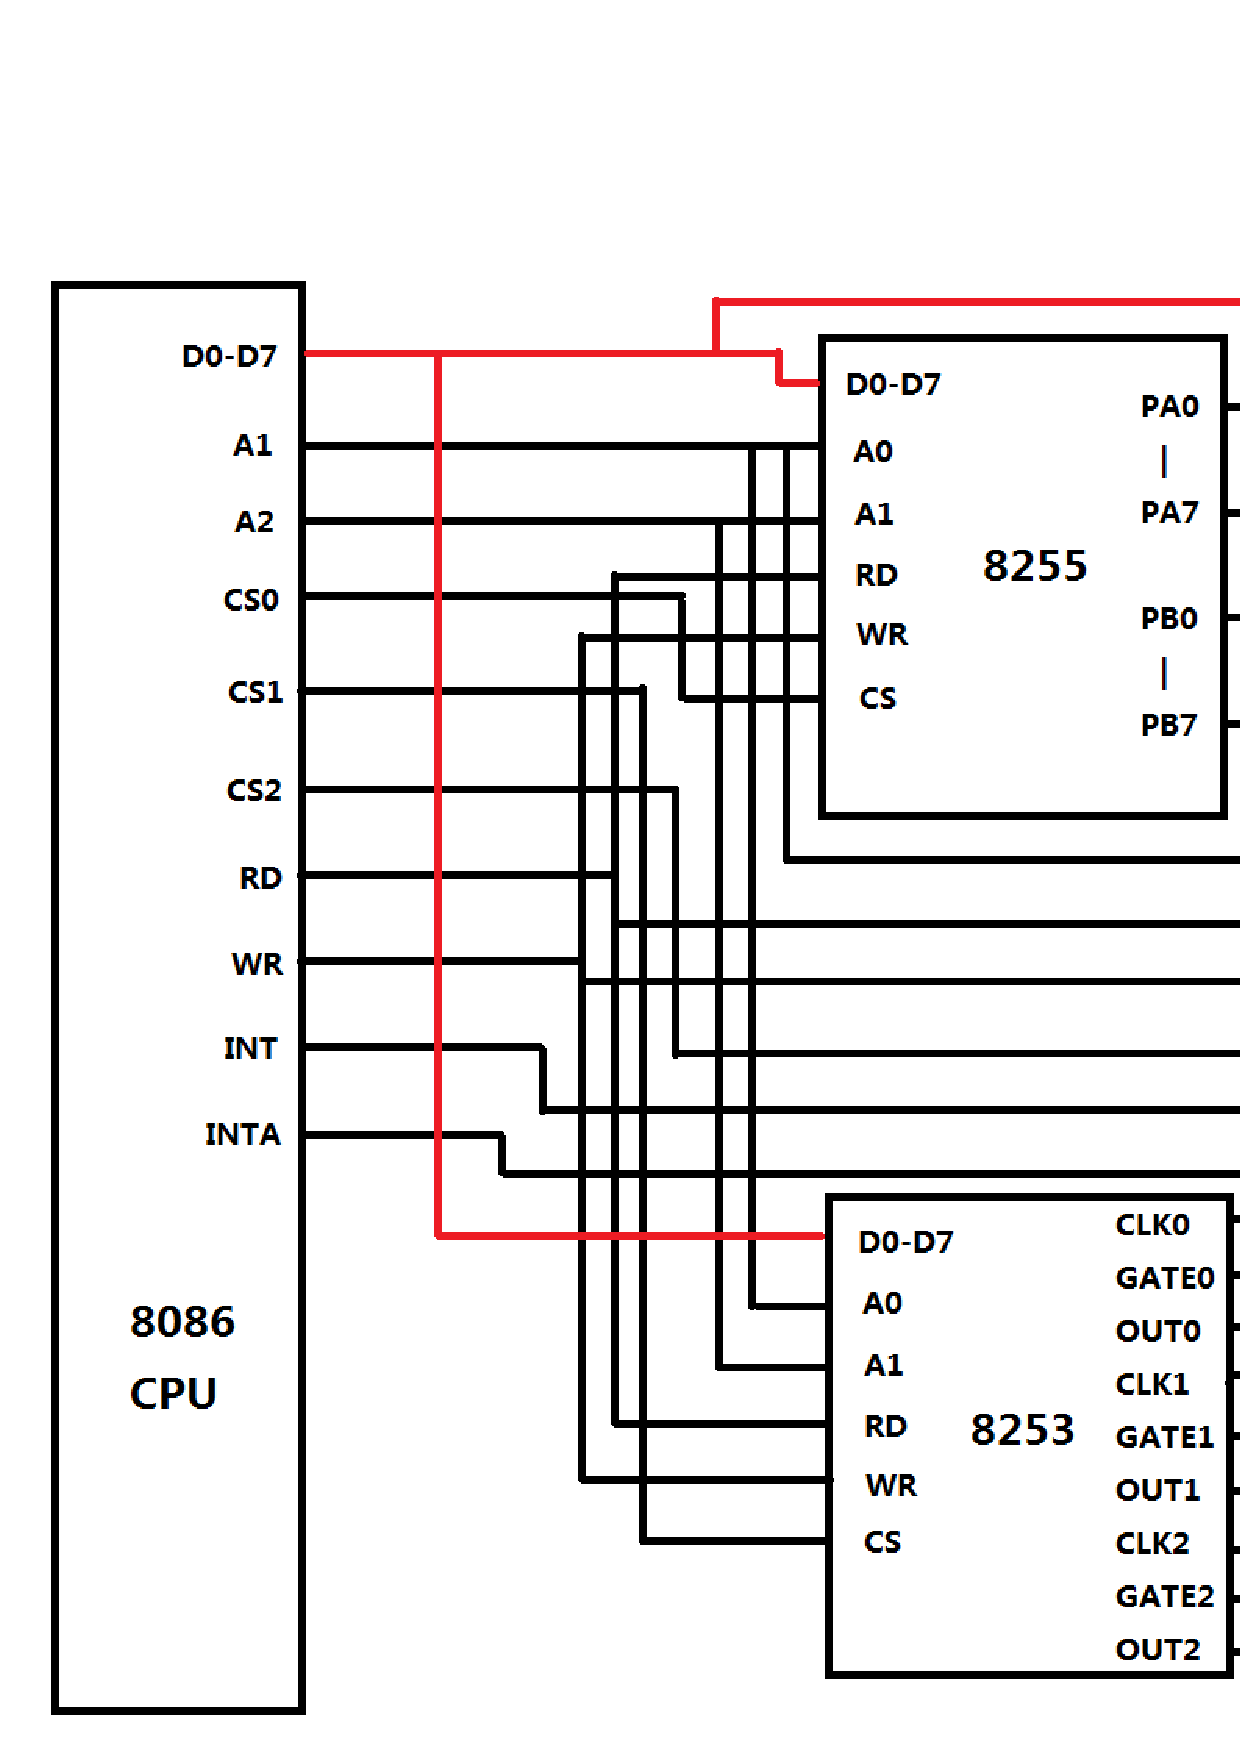
\includegraphics[width=\textwidth]{circuit.jpg}
\caption{全加器逻辑图}
\label{fig: logic}
\end{figure}
\end{center}

由全加器的真值表可写出$S_i$,$C_{i+1}$的逻辑表达式:
\begin{equation*}
\begin{aligned}
S_i&=A_i \otimes B_i \otimes C_i \\
C_{i+1}&=A_i B_i+C_i(A_i \otimes B_i)
\end{aligned}
\end{equation*}

\section{实验内容}
\begin{enumerate}
\item 用VHDL语言设计全加器。
\item 用元件例化方法设计一个四位二进制加法器。
\end{enumerate}

\section{实验设备}
\begin{enumerate}
\item 清华同方PⅣ 2.4G/256M60G
\item ISE 6.2i—Windows软件系统
\end{enumerate}

%\section{实验步骤}

\section{实验程序}
全加器代码清单如下(代码清单~\ref{lst: aonelst} )
\begin{center}
\begin{lstlisting}[caption = {全加器代码清单}, label = {lst: aonelst}]
library IEEE;
use IEEE.STD_LOGIC_1164.ALL;
use IEEE.STD_LOGIC_ARITH.ALL;
use IEEE.STD_LOGIC_UNSIGNED.ALL;

--  Uncomment the following lines to use the declarations that are
--  provided for instantiating Xilinx primitive components.
--library UNISIM;
--use UNISIM.VComponents.all;

entity aone is
port(a, b, cin: in std_logic;
	sum, cout: out std_logic);
end aone;

architecture Behavioral of aone is

begin

sum<=(a xor b) xor cin;
cout<= (a and b) or ((a xor b) and cin);

end Behavioral;
\end{lstlisting}
\end{center}

4位加法器代码清单如下(代码清单~\ref{lst: addernlst} )
\begin{center}
\begin{lstlisting}[caption = {4位加法器代码清单}, label = {lst: addernlst}]
library IEEE;
use IEEE.STD_LOGIC_1164.ALL;
use IEEE.STD_LOGIC_ARITH.ALL;
use IEEE.STD_LOGIC_UNSIGNED.ALL;

--  Uncomment the following lines to use the declarations that are
--  provided for instantiating Xilinx primitive components.
--library UNISIM;
--use UNISIM.VComponents.all;

entity addern is
port(a, b: in std_logic_vector(4 downto 1);
	cin: in std_logic;
	sum: out std_logic_vector(4 downto 1);
	cout: out std_logic);
end addern;

architecture Behavioral of addern is

component aone
port(a: in std_logic;
	b: in std_logic;
	cin: in std_logic;
	sum: out std_logic;
	cout: out std_logic);
end component;

signal carry: std_logic_vector(0 to 4);

begin

carry(0)<=cin;
cout<=carry(3);

gen: for i in 1 to 4 generate
add: aone port map(
	a=>a(i),
	b=>b(i),
	cin=>carry(i-1),
	sum=>sum(i),
	cout=>carry(i)
);	   
end generate;

end Behavioral;
\end{lstlisting}
\end{center}

\section{仿真结果}
\begin{center}
\begin{figure}[h!]
\includegraphics[width=\textwidth]{adder.jpg}
\caption{4位加法器仿真波形图}
\label{fig: cfig}
\end{figure}
\end{center}

\end{CJK*}
\end{document}
